\documentclass{beamer}
% Use DS9 global theme
\usepackage{../../../shared/templates/ds9_theme}

% Title page configuration
\title[PHYS12 CH7.1-7.3]{Work and Energy}
\subtitle{Chapter 7.1-7.3}
\author[Mr. Gullo]{Mr. Gullo}
\date[Nov 2024]{November 2024}

% Add logo
\logo{
\includegraphics[width=0.1\linewidth]{phys12-shared-cinec-logo.png}}

% Table of contents at the beginning of each section
\AtBeginSection[]
{
  \begin{frame}
    \frametitle{Table of Contents}
    \tableofcontents[currentsection]
  \end{frame}
}

\begin{document}

\frame{\titlepage}

\section{7.1 Work: The Scientific Definition}

\begin{frame}
\frametitle{Work: Definition}
\begin{itemize}
    \item Work is the transfer of energy by a force acting on an object as it is displaced
    \pause
    \item Mathematical definition: $W = F d \cos\theta$
    \pause
    \item Where:
    \begin{itemize}
        \item $W$ is work (measured in joules, J)
        \pause
        \item $F$ is force (in newtons, N)
        \pause
        \item $d$ is displacement (in meters, m)
        \pause
        \item $\theta$ is angle between force and displacement
    \end{itemize}
\end{itemize}
\end{frame}

\begin{frame}
\frametitle{Work: Important Points}
\begin{itemize}
    \item Work is zero when:
    \begin{itemize}
        \item Force and displacement are perpendicular ($\theta = 90°$)
        \pause
        \item There is no displacement ($d = 0$)
    \end{itemize}
    \pause
    \item Work is positive when:
    \begin{itemize}
        \item Force and displacement are in same direction ($\theta < 90°$)
    \end{itemize}
    \pause
    \item Work is negative when:
    \begin{itemize}
        \item Force and displacement are in opposite directions (90° < \(\theta \leq 180°\))
    \end{itemize}
\end{itemize}
\end{frame}

\section{7.2 Kinetic Energy}

\begin{frame}
\frametitle{Kinetic Energy}
\begin{itemize}
    \item Kinetic energy is the energy of motion
    \pause
    \item Formula: $KE = \frac{1}{2}mv^2$
    \pause
    \item Where:
    \begin{itemize}
        \item $m$ is mass (kg)
        \pause
        \item $v$ is velocity (m/s)
    \end{itemize}
    \pause
    \item Work-Energy Theorem: $W_{net} = \Delta KE$
    \pause
    \item Net work equals change in kinetic energy
\end{itemize}
\end{frame}

\section{7.3 Gravitational Potential Energy}

\begin{frame}
\frametitle{Gravitational Potential Energy}
\begin{itemize}
    \item Energy due to position in a gravitational field
    \pause
    \item Formula: $PE_g = mgh$
    \pause
    \item Where:
    \begin{itemize}
        \item $m$ is mass (kg)
        \pause
        \item $g$ is acceleration due to gravity (9.8 m/s²)
        \pause
        \item $h$ is height (m)
    \end{itemize}
    \pause
    \item Depends only on vertical height change
    \pause
    \item Reference level can be chosen arbitrarily
\end{itemize}
\end{frame}


\begin{frame}
\begin{columns}[T]
    % Left column
    \begin{column}{0.5\textwidth}
        \begin{figure}
            \centering
            
\includegraphics[width=0.7\linewidth]{Screenshot 2024-11-19 071730.png}
        \end{figure}
        \begin{figure}
            \centering
            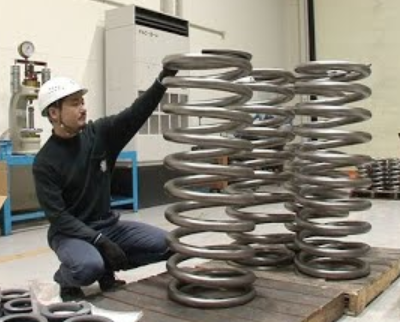
\includegraphics[width=0.7\linewidth]{Screenshot 2024-11-19 073518.png}
        \end{figure}
    \end{column}
    
    % Right column
    \begin{column}{0.5\textwidth}
        \begin{figure}
            \centering
            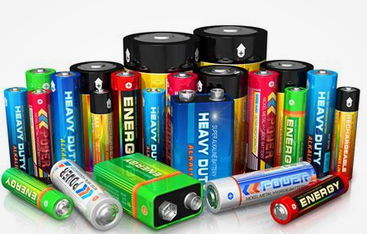
\includegraphics[width=0.7\linewidth]{phys12-circuits-kirchhoffs-loop-rule-example.png}
        \end{figure}
        \begin{figure}
            \centering
            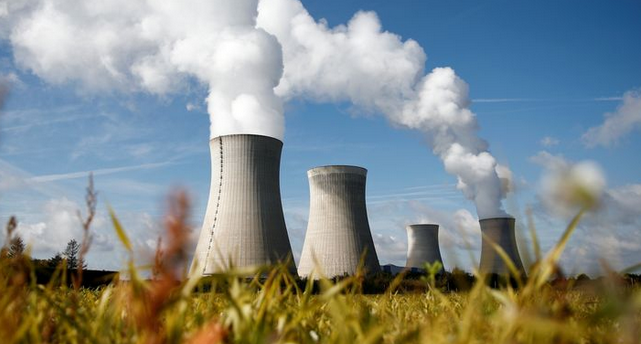
\includegraphics[width=0.7\linewidth]{Screenshot 2024-11-19 074004.png}
        \end{figure}
    \end{column}
\end{columns}
\end{frame}

\section{Example Problems}

\begin{frame}
\frametitle{Example 7.1: Calculating Work You Do to Push a Lawn Mower}
A person pushing a lawn mower exerts a constant force of 75.0 N at an angle 35° below the horizontal. The lawn mower is pushed 25.0 m on level ground.
\vspace{0.5cm}
\end{frame}

\begin{frame}
\textbf{Solution:}
\begin{align*}
W &= Fd\cos\theta \\
\pause
W &= (75.0\text{ N})(25.0\text{ m})\cos(35.0°) \\
\pause
W &= 1536\text{ J} = 1.54 \times 10^3\text{ J} \\
\pause
\text{Convert to kcal:} &= 0.367\text{ kcal} \\
\pause
\text{Ratio to daily intake:} &= 1.53 \times 10^{-4}
\end{align*}
\end{frame}

\begin{frame}
\frametitle{Example 7.2: Calculating the Kinetic Energy of a Package}
A 30.0-kg package on a roller belt conveyor system moves at 0.500 m/s.
\vspace{0.5cm}
\end{frame}

\begin{frame}
\textbf{Solution Steps:}
\begin{enumerate}
    \item KE = $\frac{1}{2}mv^2$ 
    \pause
    \item KE = $0.5(30.0\text{ kg})(0.500\text{ m/s})^2$
    \pause
    \item KE = $3.75\text{ kg}\cdot\text{m}^2/\text{s}^2 = 3.75\text{ J}$
\end{enumerate}
\end{frame}

\begin{frame}
\frametitle{Example 7.7: Finding the Speed of a Roller Coaster from its Height}
(a) What is the final speed of the roller coaster shown in the text if it starts from rest at the top of the 20.0 m hill and work done by frictional forces is negligible?

\begin{figure}[H]
    \centering
    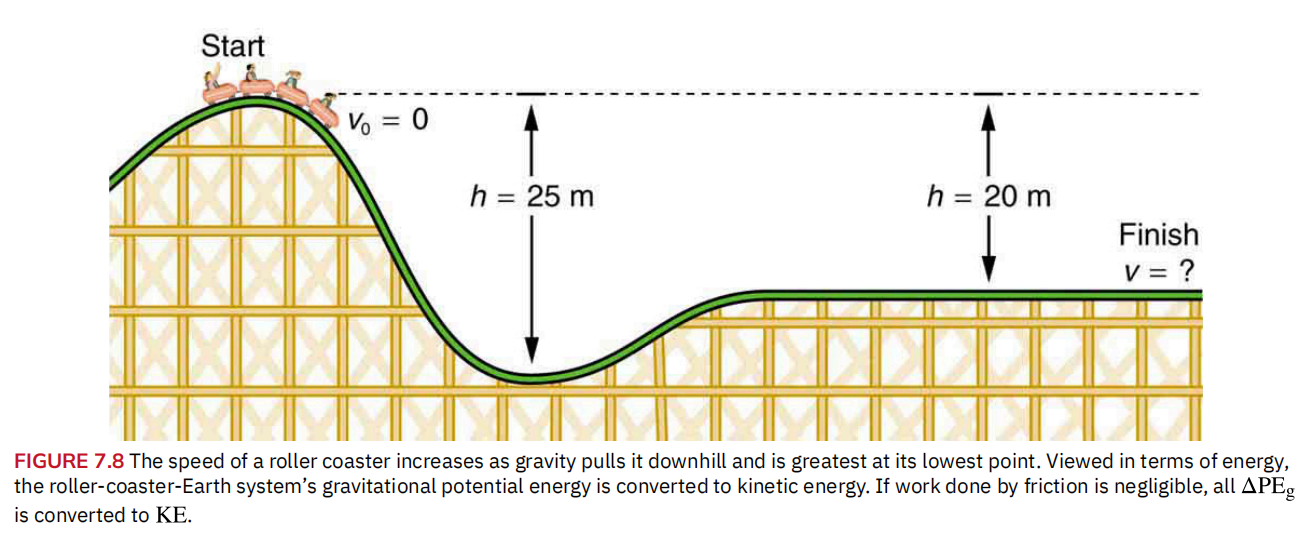
\includegraphics[width=0.75\linewidth]{Screenshot 2024-11-19 090237.png}
\end{figure}
Try this on your own, then we'll discuss the solution!
\end{frame}

\begin{frame}{ex. 7.7}
    

(b) What is its final speed (again assuming negligible friction) if its initial speed is 5.00 m/s?

\begin{figure}[H]
    \centering
    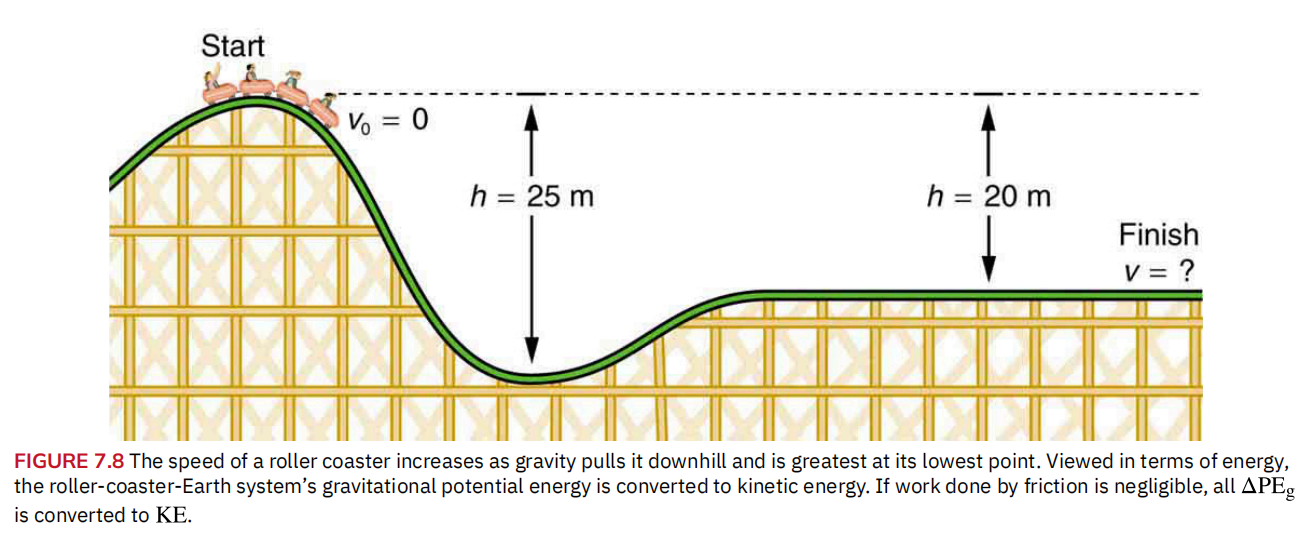
\includegraphics[width=0.75\linewidth]{Screenshot 2024-11-19 090237.png}
\end{figure}
Try this on your own, then we'll discuss the solution!
\end{frame}

\begin{frame}
\frametitle{You Do: Solution}
\textbf{Solution:}
\begin{align*}
\text{For (a):} \\
\pause
v &= \sqrt{2g|h|} \\
\pause
v &= \sqrt{2(9.80\text{ m/s}^2)(20.0\text{ m})} \\
\pause
v &= 19.8\text{ m/s} \\
\\
\pause
\text{For (b):} \\
\pause
v &= \sqrt{2g|h| + v_0^2} \\
\pause
v &= \sqrt{2(9.80)(20.0) + (5.00)^2} \\
\pause
v &= 20.4\text{ m/s}
\end{align*}
\end{frame}

\begin{frame}
\frametitle{Example 7.7: Discussion}
\begin{itemize}
    \item Mass cancels out - consistent with all objects falling at same rate
    \pause
    \item Speed depends only on initial speed and height
    \pause
    \item Path taken doesn't matter - only initial and final heights
    \pause
    \item Final speed in (b) greater but by less than the initial 5.00 m/s
\end{itemize}

\end{frame}

\begin{frame}{Key Principles}
\begin{block}{Key Principle}
In a system with only conservative forces:
\[E_{\text{total}} = \text{KE} + \text{PE} = \text{constant}\]
\end{block}
\pause

\begin{block}{Mathematical Expression}
\[\text{KE}_i + \text{PE}_i = \text{KE}_f + \text{PE}_f\]
Where:
\begin{itemize}
\item \(\text{KE} = \frac{1}{2}mv^2\) (Kinetic Energy)
\item \(\text{PE} = mgh\) (Gravitational Potential Energy)
\end{itemize}
\end{block}
\pause

\begin{alertblock}{Important Notes}
\begin{itemize}
\item Energy can transform between KE and PE
\pause
\item Total mechanical energy is conserved
\pause
\item Valid only for conservative forces
\end{itemize}
\end{alertblock}
\end{frame}

\end{document}